%-----------------------------------------------------------------------------
%
%               Template for sigplanconf LaTeX Class
%
% Name:         sigplanconf-template.tex
%
% Purpose:      A template for sigplanconf.cls, which is a LaTeX 2e class
%               file for SIGPLAN conference proceedings.
%
% Guide:        Refer to "Author's Guide to the ACM SIGPLAN Class,"
%               sigplanconf-guide.pdf
%
% Author:       Paul C. Anagnostopoulos
%               Windfall Software
%               978 371-2316
%               paul@windfall.com
%
% Created:      15 February 2005
%
%-----------------------------------------------------------------------------


\documentclass{sigplanconf}

% The following \documentclass options may be useful:

% preprint      Remove this option only once the paper is in final form.
% 10pt          To set in 10-point type instead of 9-point.
% 11pt          To set in 11-point type instead of 9-point.
% authoryear    To obtain author/year citation style instead of numeric.

\usepackage{amsmath}

\usepackage{graphicx}
\graphicspath{ {images/} } % Path to images folder

\begin{document}

\special{papersize=8.5in,11in}
\setlength{\pdfpageheight}{\paperheight}
\setlength{\pdfpagewidth}{\paperwidth}

\conferenceinfo{CONF '14}{September 29, 2014, 2014, Golden, CO, USA} 
\copyrightyear{2014} 
\copyrightdata{978-1-nnnn-nnnn-n/yy/mm} 
\doi{nnnnnnn.nnnnnnn}

% Uncomment one of the following two, if you are not going for the 
% traditional copyright transfer agreement.

%\exclusivelicense                % ACM gets exclusive license to publish, 
                                  % you retain copyright

%\permissiontopublish             % ACM gets nonexclusive license to publish
                                  % (paid open-access papers, 
                                  % short abstracts)

\titlebanner{banner above paper title}        % These are ignored unless
\preprintfooter{short description of paper}   % 'preprint' option specified.

\title{GPU-Based Parallel Finite State Machines}

\authorinfo{Kameron W. Kincade\and Ryan P. Langewisch}
           {Colorado School of Mines}
           {kkincade@mines.edu | rlangewi@mines.edu}

\maketitle

%\begin{abstract}
%Abstract goes here.
%\end{abstract}

% general terms are not compulsory anymore, 
% you may leave them out
\terms
finite state machines, GPU, parallelization

\section{Introduction}

A finite state machine (FSM) is used to represent an object that can exist in a limited number of states and that can change state based on a number of well-defined rules (Figure 1). Each FSM is responsible for processing various inputs (each usually represented as a string of characters) and determining if these inputs satisfy the machine's acceptance criteria, represented by ending in one of the machine's final states. To operate on an input string, the FSM begins with the start state (A in Figure 1) and processes each character one after another. The state machine's transition rules, along with the input character, dictate the next location to move to. An acceptance state (D) is commonly indicated by a double circle and represents a valid input solution that satisfies the FSM's criteria.

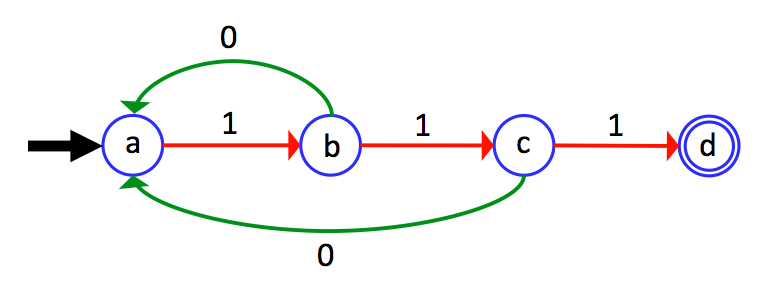
\includegraphics[width=\linewidth]{fsm_diagram.png}

FSMs are embedded in many different types of applications, including web application computations such as lexing, parsing, translations, and media encoding/decoding. With the recent emphasis on mobile, handheld devices, the need for a computationally efficient implementation of FSMs is becoming more important. Parallelization is one of the obvious ways to speed up the execution of a program. However, the exclusively sequential execution of FSM's also make them difficult to parallelize. The most evident way to parallelize a FSM is to divide the input string into a number of different FSM input strings, known as substrings, each of which can be processed in parallel. The problem with this approach is determining the start state for each new substring. The start state of one substring should be the end state of the previous substring, but due to the nature of FSMs, this state is unknown until the previous substring has completely finished processing. One approach is to make an educated guess for the start state. This paper describes a proposed method to make this educated guess, along with a parallelization technique to utilize the processing power provided by GPUs.

\section{Previous Work and Goal}
The topic of parallelizing FSM's is a relatively new area of research. Two papers were specifically studied in order to understand the current progress made in this field: \textit{Challenging the "Embarassingly Sequential": Parallelizing Finite State Machine-Based Computations through Principled Speculation} by a group from the College of William and Mary, and \textit{Data-Parallel Finite-State Machines} by a group from Microsoft. Both of these papers explored techniques for improving the performance of FSM processing on CPU, but did not apply their findings to GPU. It is this fact that leads us to the primary goal for our project: \textbf{Our goal is to implement deterministic finite state machines on GPU}. Our approach will consist of initially just getting an implementation working without optimization, and then add in modular layers of optimization such as the techniques discussed in the above papers. This goal is challenging for many of the same reasons as FSM on CPU; it is about as sequential as a process could be, which makes it a very interesting challenge to parallelize, requiring a different approach than typical parallel programs. There is also added interest due to the fact that FSM's have yet to be implemented on GPU, making any progress in the focused area a step into new territory of research.


\section{Methods}

To achieve our goal of implementing FSM processing in parallel on GPU, there are specific methods from the previous research that we will attempt to implement. In efforts to correctly guess the start state of a substring, a technique known as lookback is utilized. Lookback involves analyzing a certain number of input characters prior to the start of the particular substring. The advantage of lookback lies in the context provided by analyzing the previous input characters. This context might eliminate a number of states from being possible start states due to the nature and structure of the FSM. As a result, this increases the chances of choosing the correct start state for a given substring. A couple subjects of research include how many substrings to divide the original input string into, how many lookback characters to analyze, and how the number of available processors influences the execution time of a given parallelized FSM.

Beyond the concept of lookback, additional steps can be taken to try and decrease the execution time of a parallelized FSM. To fully utilize the number of cores on a GPU, a parallel FSM implementation can use an enumerative approach when it is unsure of the start state for a particular substring. The enumerative approach begins calculating all possible paths for the FSM. Once a correct start state is found, the correct path from the multiple, enumerated paths is used as part of the solution for the state machine. To make the enumerative approach more efficient, when a start state is correctly identified, all unfinished subprocesses using incorrect start states are terminated to make room for more subprocesses to begin.

Particularly in the research paper by the group from the College of William and Mary, there was an emphasis on profiling of the FSM prior to the actual parallel computation. For the purposes of our implementation strategy, we are first going to assume no profiling and try to optimize the algorithm's ability to efficiently deduce information about the FSM as it is running. That said, we plan to keep our design very open in order that a strategy such as profiling could easily be explored and added in the future if we decide that it would be a useful addition and a logical next step in our implementation process.

\section{Tools and Approach}
The objective of the GPU-based implementation is to be compatible with any type of GPU. This could range from a small GPU inside a laptop machine and could extend to a larger, much more powerful GPU containing thousands of cores. Specifically, the code will be executed on a few different machines: a Macbook Pro containing a 16 core NVIDIA GeForce 9400M, a desktop machine using a NVIDIA GeForce GTX 650 Ti Boost, and a Colorado School of Mines server with a much more powerful GPU. The results of each GPU will be analyzed to help better understand the possible effects of the number of cores on an FSM implementation.

All of the subjected GPUs are listed as compatible devices with the CUDA (Compute Unified Device Architecture) language, which is the language that will be used in the implementation. CUDA is a parallel programming language initially developed by NVIDIA as an extension of the C language. It now has extensions for C++ and Fortran as well. The CUDA language provides an additional set of keywords and methods to help parallelize programs for use with general purpose processing on graphical processing units (GPGPU), rather than actual graphical processing purposes.

Having no experience with the CUDA language, the first step in our approach is going to consist of becoming more familiar with developing on GPU through that medium. Once we have a handle on the structuring of CUDA programs, our next goal will be to develop a bare-bone implementation of FSM through CUDA. This first iteration will not focus on optimization, but rather just get something that actually runs successfully on GPU. Implementing this base functionality is something that we hope to have finished, or at least investigated thoroughly, by the project milestone. The development beyond the project milestone is going to be intentionally left open to be modified on the fly. We are unsure at this point where our research and development will take us, and we want to to stay open to the possibility of extending the project into the future rather than cutting it short to make a deadline at the end of the semester. Whatever the case, this development will consist of applying techniques such as those found in the reference research papers, and combining them with our own approach in the hopes of creating an implementation that specifically is tailored towards GPU and yields results that take advantage of the processing power and parallelization that GPU provides.

%\appendix
%\section{Appendix Title}

%This is the text of the appendix, if you %need one.

%\acks

%Acknowledgments, if needed.

% We recommend abbrvnat bibliography style.

%\bibliographystyle{abbrvnat}

% The bibliography should be embedded for final submission.

%\begin{thebibliography}{}
%\softraggedright

%\bibitem[Smith et~al.(2009)Smith, Jones]%{smith02}
%P. Q. Smith, and X. Y. Jones. %...reference text...

%\end{thebibliography}


\end{document}

%                       Revision History
%                       -------- -------
%  Date         Person  Ver.    Change
%  ----         ------  ----    ------

%  2013.06.29   TU      0.1--4  comments on permission/copyright notices

